\documentclass{beamer}
\usetheme[pageofpages=of,% String used between the current page and the
                         % total page count.
          bullet=circle,% Use circles instead of squares for bullets.
          titleline=true,% Show a line below the frame title.
          alternativetitlepage=true,% Use the fancy title page.
       %   titlepagelogo=logo-polito,% Logo for the first page.
       %   watermark=watermark-polito,% Watermark used in every page.
       %   watermarkheight=100px,% Height of the watermark.
       %   watermarkheightmult=4,% The watermark image is 4 times bigger
                                % than watermarkheight.
          ]{Torino}

\setbeamertemplate{footline}{
  \begin{beamercolorbox}[wd=\paperwidth,ht=1ex,dp=1ex]{footline}
    \vspace{5pt} \hspace{1em} \insertframenumber/\inserttotalframenumber
  \end{beamercolorbox}
}

\author{Brendon J. Brewer}
\title{STATS 331 -- Introduction to Bayesian Statistics}
\institute{The University of Auckland}
\date{}


\linespread{1.3}
\usepackage{minted}
\usepackage[utf8]{inputenc}
\usepackage{dsfont}
\newcommand{\given}{\,|\,}
\newcommand{\balpha}{\boldsymbol{\alpha}}
\newcommand{\bmu}{\boldsymbol{\mu}}


\begin{document}

\frame{\titlepage}

\begin{frame}
\begin{center}
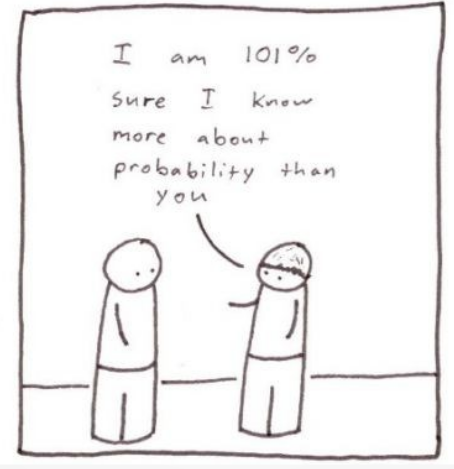
\includegraphics[width=0.6\textwidth]{images/101.png}

Credit: www.afewpanels.com
\end{center}

\end{frame}


\begin{frame}
\Large

\begin{center}
Time Series Models
\end{center}
\end{frame}

\begin{frame}
\frametitle{Poll}
How many of you have studied a course involving `time series models'
such as the AR(1)?
\end{frame}


\begin{frame}
\frametitle{What is a Time Series}
There are two related meanings for the term {\bf time series}.

\begin{itemize}
\item [(1)] Any quantity that varies over time.
\end{itemize}

\begin{center}
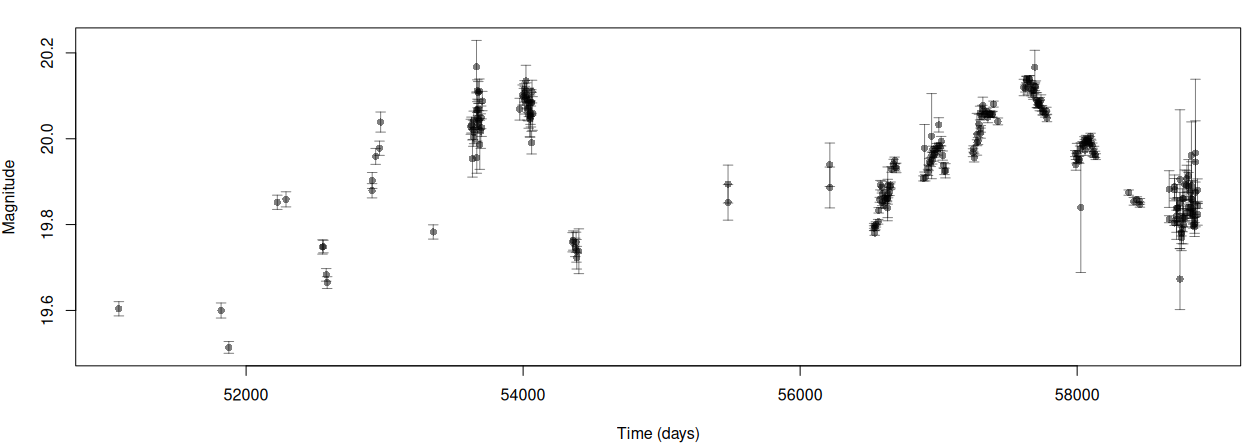
\includegraphics[width=0.9\textwidth]{images/time_series.png}
\end{center}

\end{frame}

\begin{frame}
\frametitle{What is a Time Series}
There are two related meanings for the term {\bf time series}.

\begin{itemize}
\item [(2)] A {\bf probability distribution} for a quantity that varies over time.\pause
\item That is, not any single curve, but a probability distribution over the
set of possible curves.
\end{itemize}

\end{frame}

\end{document}

